%A natural question when considering the performance of a neural network is whether, or to what extent, the hyperparameters must be modified to achieve good performance on a new dataset. Jiffy's consistent performance across the above datasets using fixed hyperparameters suggests that little modification is required. To assess this further, however, we measured the changes in Jiffy's performance on additional datasets while varying two parameters that were especially likely to affect performance in early experiments---the embedding size and the amount of maxpooling.

A natural question when considering the performance of a neural network is whether, or to what extent, the hyperparameters must be modified to achieve good performance on a new dataset. In this section, we explore the robustness of our approach with respect to the values of the two key parameters: embedding size and pooling percentage. We do this by learning metrics for a variety of parameter values for ten data sets from the UCR Time Series Archive \citep{ucrArchive}, and evaluating how classification accuracy varies.

%Jiffy's consistent performance across the above datasets using fixed hyperparameters suggests that little modification of th is required, but to assess this further, we run

%Because they are widely used, we chose 10 datasets at random from the UCR time series archive \cite{ucrArchive}.

% In the interest of exploring the stability of our model's performance with respect to parameter choice without tuning our network to the test datasets, we rigorously test parameter choices against a suite of 10 datasets from the UCR Time Series Archive. We explore two parameters in particular: embedding size and pooling percentage.

% ================================
\subsection{Embedding Size}
% ================================

%The plot on the left of Figure \ref{fig:params} 
Figure \ref{fig:params}.\textit{left} shows that even a few dozen neurons are sufficient to achieve peak accuracy. As a result, an embedding layer of 40 neurons is sufficient and leads to an architecture that is compact enough to run on a personal laptop.

% It is apparent that after a certain point additional neurons have little to no effect in the utility of the embedding for classification.

\begin{figure}[h]
\begin{center}
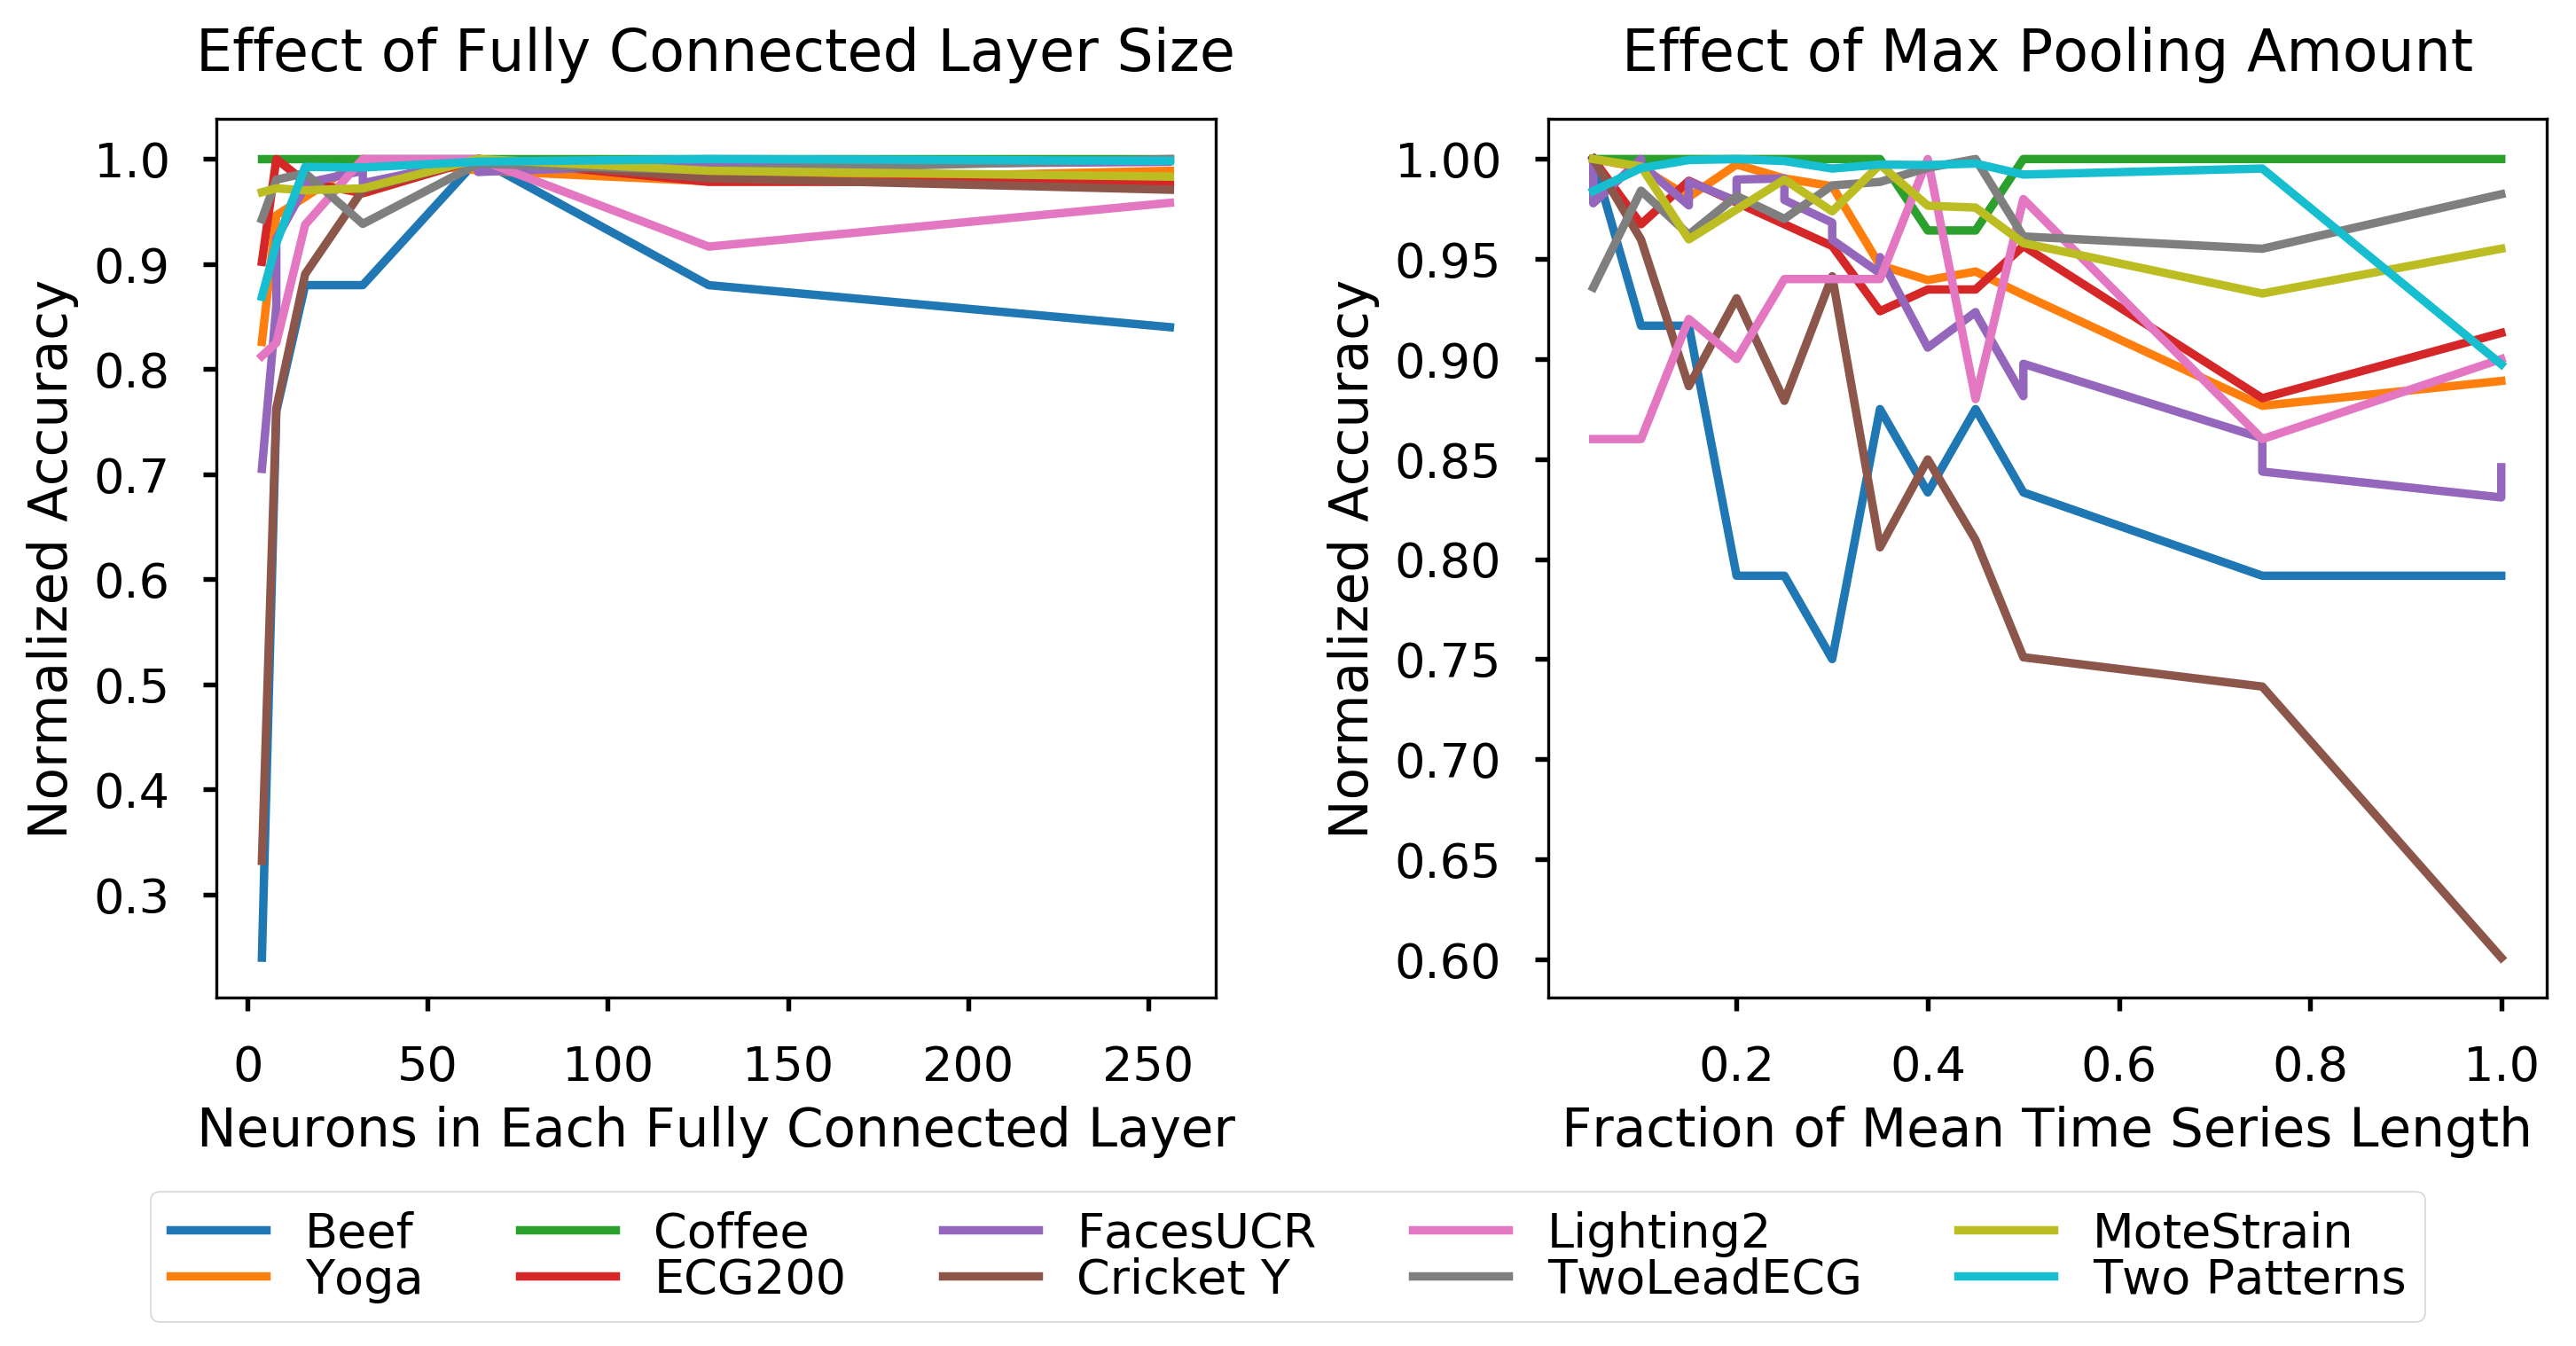
\includegraphics[width=\linewidth]{param_effects}
\vspace*{-5mm}
\caption{Effect of fully connected layer size and degree of max pooling on model accuracy using held-out datasets. Even small fully connected layers and large amounts of max pooling---up to half of the length of the time series in some cases---have little or no effect on accuracy. For ease of visualization, each dataset's accuracies are scaled such that the largest value is 1.0.}
\label{fig:params}
\end{center}
\end{figure}

% ================================
\subsection{Pooling percentage}
% ================================
% This method is especially common in shapelet-based classification procedures in which a candidate shapelet is convolved across the entire time series in an attempt to find the closest distance between the given shapelet and a subsequence of the time series.

The typical assumption in machine learning literature is that max pooling windows in convolutional architectures should be small to limit information loss. In contrast, time series algorithms often max pool globally across each example (e.g. \citep{learningShapelets}). Contrary to the implicit assumptions of both, we find that the level of pooling that results in the highest classification often falls in the 10-25\% range, as shown by Figure \ref{fig:params}.\textit{right} % the plot on the right side of Figure \ref{fig:params}.

% \subsection{Unsupervised Learning}

% % ================================
% \subsubsection{Embedding Size}
% % ================================
% In line with our observation in the supervised setting, we see (Figure~\ref{fig:params_unsupervised}) that embedding size has little to no effect on the quality of the autoencoder architecture's produced clustering. This aligns with our understanding of time series data; each of these datasets is inherently low dimensional and the negligible clustering purity increase as the embedding size grows reflects that.

% % ================================
% \subsubsection{Pooling Percentage}
% % ================================
% We observe a similar phenomenon to the supervised setting in that we are able to pool broadly at no cost to the resulting cluster purity (Figure ~\ref{fig:params_unsupervised}). This behavior contradicts previous approaches to pooling over time series; other methods use globally averaged filters or fixed width windows. 

% \begin{figure}[h]
% \begin{center}
% 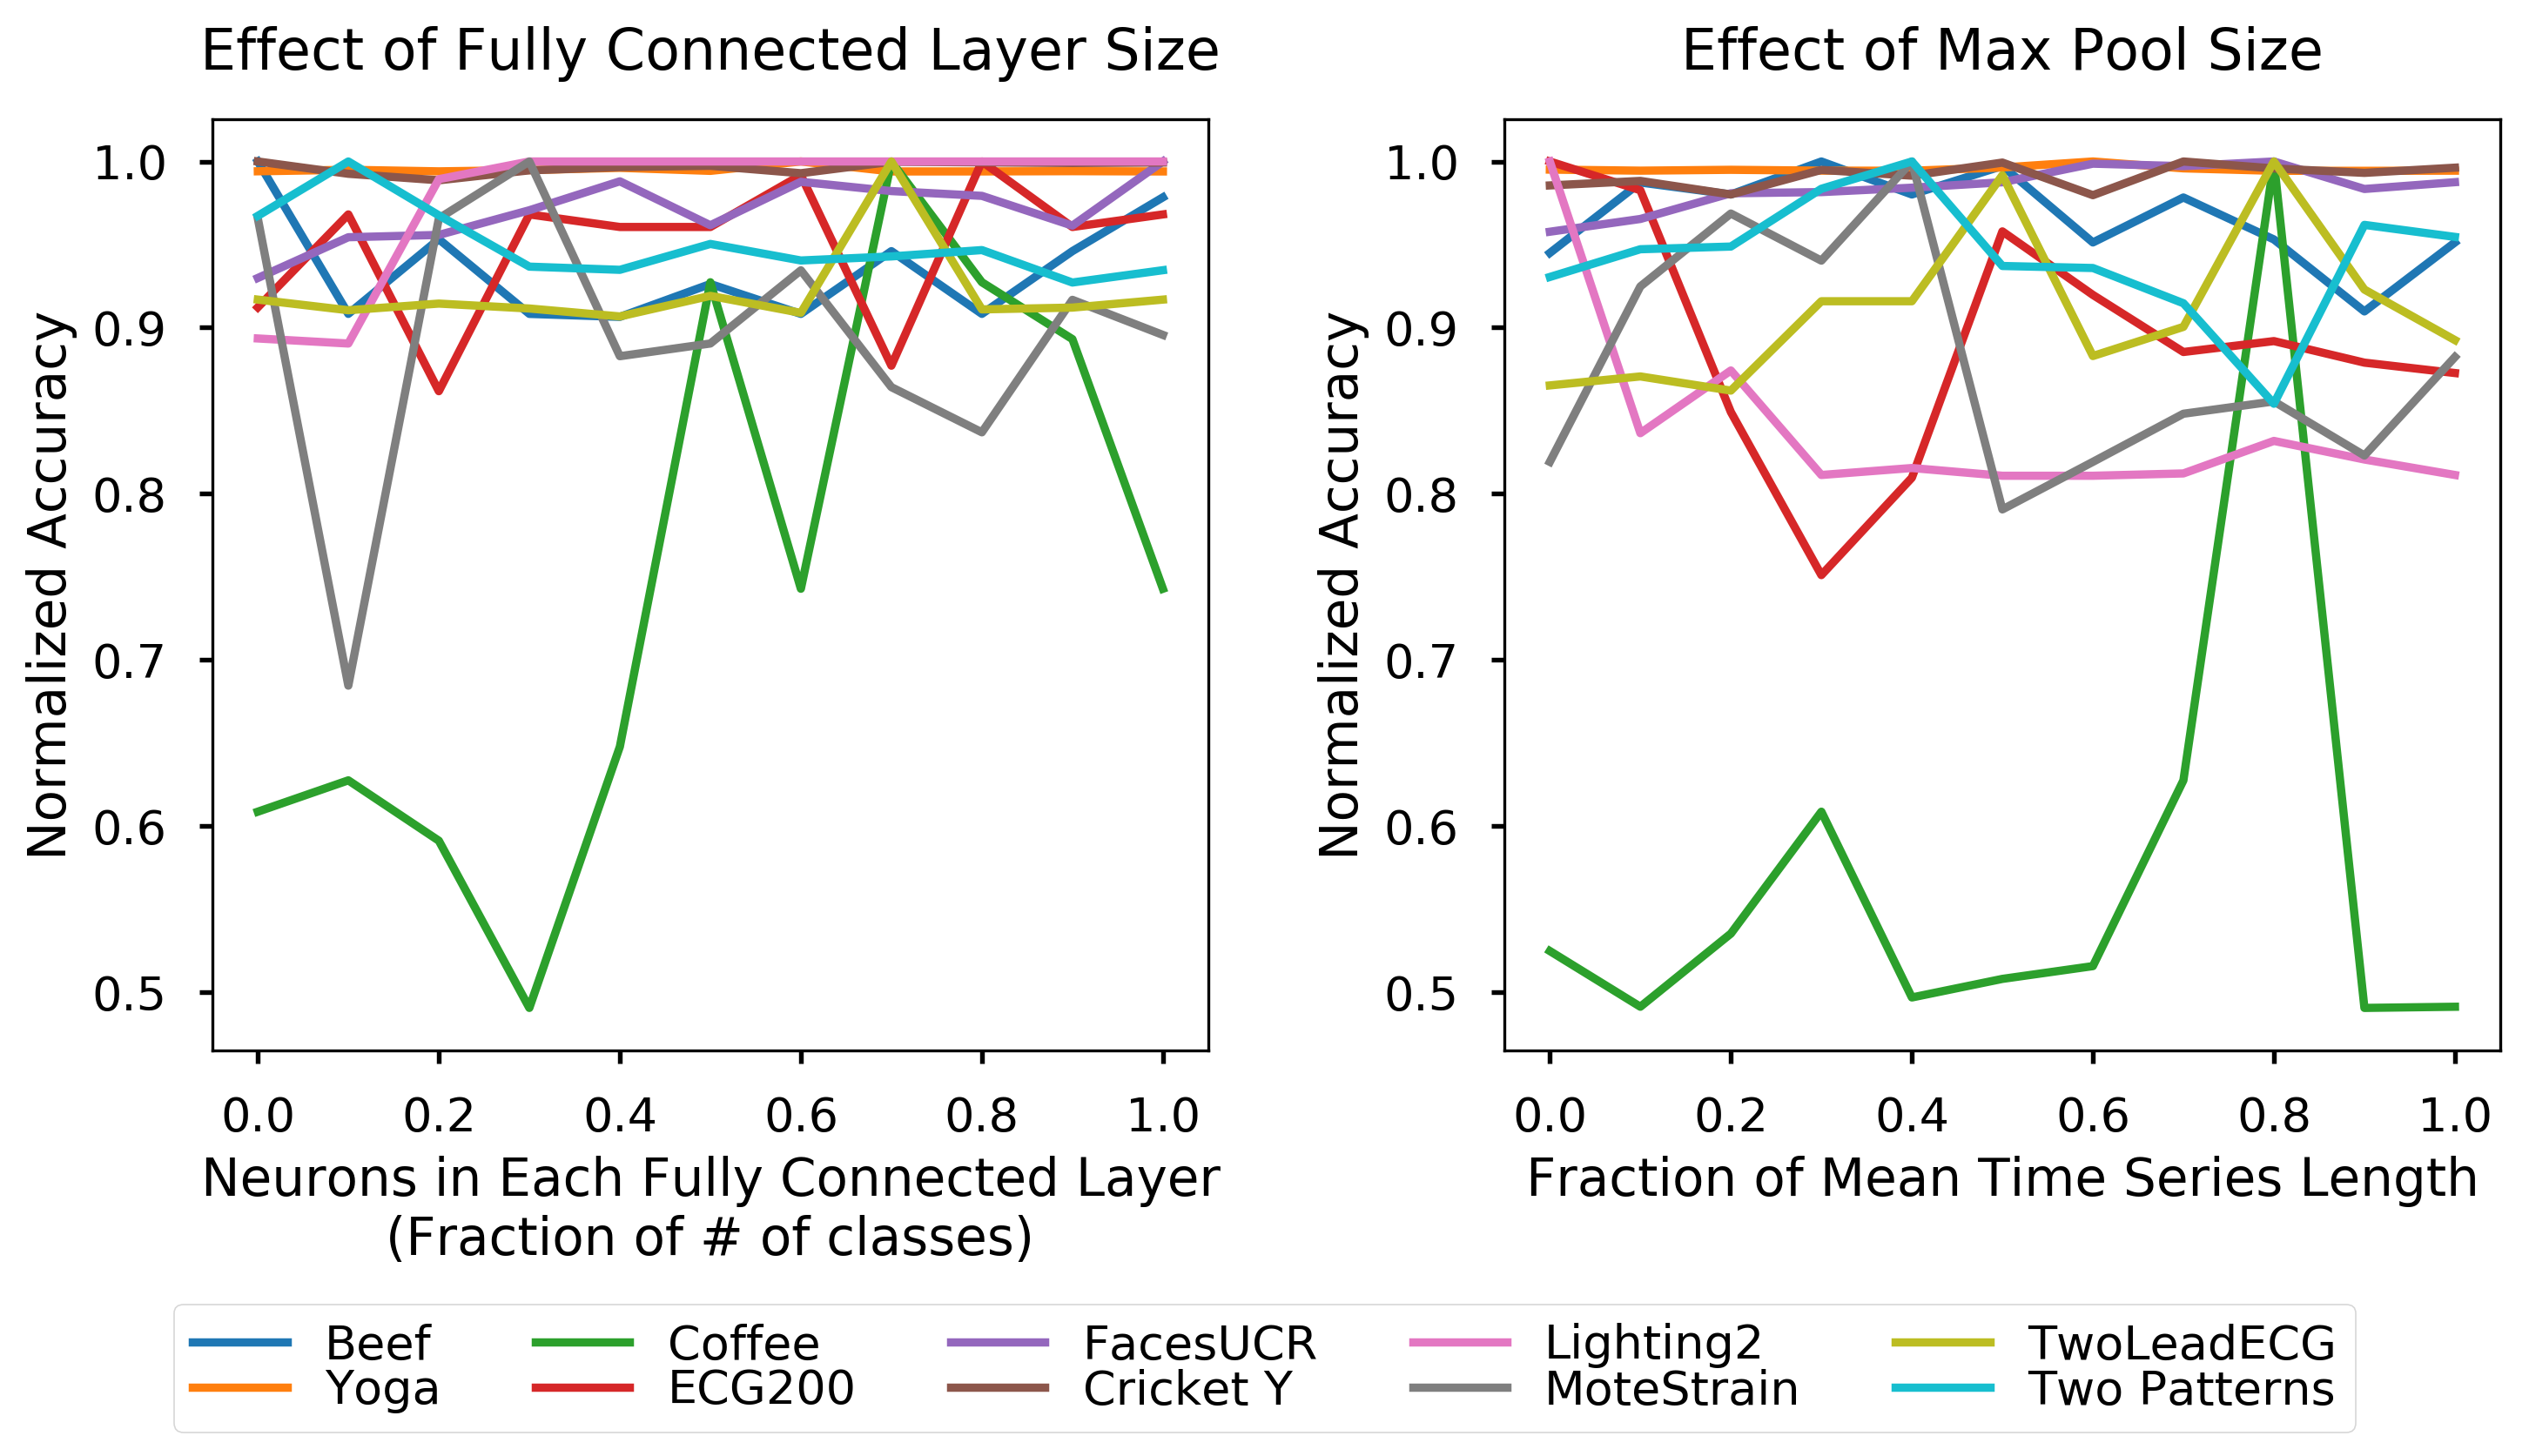
\includegraphics[width=\linewidth]{param_effects_unsupervised}
% \vspace*{-5mm}
% \caption{Effect of fully connected layer size and degree of max pooling on model accuracy using held-out datasets. Even small fully connected layers and large amounts of max pooling---up to half of the length of the time series in some cases---have little or no effect on accuracy. For ease of visualization, each dataset's accuracies are scaled such that the largest value is 1.0.}
% \label{fig:params_unsupervised}
% \end{center}
% \end{figure}



